% -----------------------------------------------
% Template for ISMIR 2014
% (based on earlier ISMIR templates)
% -----------------------------------------------

\documentclass{article}
\usepackage{ismir2014,amsmath,cite}
\usepackage{graphicx}
\usepackage{amsfonts}
\usepackage{brian}
\usepackage{qtree}
\usepackage{caption}
\usepackage{subcaption}
\def\shag{\ensuremath{\text{\textsc{SHAG}}}}
\DeclareMathAlphabet{\mathpzc}{OT1}{pzc}{m}{it}

% Title.
% ------
\title{Hierarchical evaluation of music segment boundary detection}

% Single address
% To use with only one author or several with the same address
% ---------------
%\oneauthor
% {Names should be omitted for double-blind reviewing}
% {Affiliations should be omitted for double-blind reviewing}

% Two addresses
% --------------
\twoauthors
  {First author} {School \\ Department}
  {Second author} {Company \\ Address}

% Three addresses
% --------------
%\threeauthors
  %{First author} {Affiliation1 \\ {\tt author1@ismir.edu}}
  %{Second author} {\bf Retain these fake authors in\\\bf submission to preserve the formatting}
  %{Third author} {Affiliation3 \\ {\tt author3@ismir.edu}}

% Four addresses
% --------------
%\fourauthors
%  {First author} {Affiliation1 \\ {\tt author1@ismir.edu}}
%  {Second author}{Affiliation2 \\ {\tt author2@ismir.edu}}
%  {Third author} {Affiliation3 \\ {\tt author3@ismir.edu}}
%  {Fourth author} {Affiliation4 \\ {\tt author4@ismir.edu}}

\begin{document}
%
\maketitle
%
\begin{abstract}
Structure in music is traditionally analyzed hierarchically: large scale sections at the highest level can be sub-divided and refined down to the short melodic ideas at the motivic level. 
However, typical algorithmic approaches to structural annotation produce flat temporal partitions of a track, which are commonly evaluated against a similarly flat, human-produced
annotation, effectively discarding all notions of structural depth in the annotation.
Recently, collections of hierarchical structure annotations have been published, but at present, no evaluation techniques exist to evaluate against these rich structural annotations.
We propose a method to evaluate structural boundary detection in the context of hierarchical annotation.
The proposed method transforms boundary detection into a ranking problem, and facilitates the comparison of flat and hierarchical annotations.
We demonstrate the proposed method with various synthetic and real world examples. 
\end{abstract}
%
\section{Introduction}\label{sec:introduction}

The analysis of the structure in music has been one of the main areas of interest by musicologists for many years.
Its goal is to identify and categorize the form of a musical piece by investigating the organization of its components, such as sections, phrases, melodies, or recurring motives.
Traditional analyses usually provide multiple levels of annotation (\eg, Schenkerian analysis), which reinforce the general assumption that music is structured hierarchically~\cite{Lerdahl1983a}.
Consequently, tree representations are commonly used to both model and analyze hierarchical forms in music~\cite{Lerdahl1983}.

In the music information retrieval literature, \emph{music segmentation} is a task that aims to automatically identify the structure of music~\cite{Paulus2010}.
As opposed to other, more traditional approaches, the segmentation task has generally focused on partitioning a song into non-overlapping segments (or sections).
Nevertheless, it has been shown that even these segments tend to be organized in a hierarchical manner~\cite{Peeters2009}, and even a large dataset of hierarchically-structured human 
annotations is now publicly available~\cite{Smith2011}.
% Still, most existing algorithms only operate at a flat level, likely because (i) this task is already challenging at this level~\cite{Skywalker2014}, and (ii) even if an algorithm could 
% estimate hierarchical segments, no method to evaluate them has been proposed.
However, current evaluation methodologies are defined only for flat segmentations, both in the estimation (algorithm output) and reference human annotation data.  Therefore, the
dimension of \emph{depth} has been practically ignored in the evaluation of music segmentation algorithms.

%This automatic task could facilitate, e.g., the intra-piece navigation, generation of music summaries, or segment-based recommendation systems, especially nowadays when listeners have easy access to large digital music collections.
%Nevertheless, the vast majority of music segmentation algorithms only operate at a flat level instead of following the hierarchical approach that most musicologists follow.

In this work we present the \emph{Segment Hierarchy Agreement Grades} (SHAG), a method to evaluate the accuracy of boundaries in hierarchical segmentations.
The proposed metric works at a frame-level --- similar to the method of Levy and Sandler~\cite{Levy2008}, a score used to evaluate structural annotations --- and it is based on a rank retrieval evaluation where each frame is ranked depending on whether it belongs to the \emph{correct} segment.
The correctness of the segment is evaluated simultaneously across all hierarchical layers, thus resulting in a metric that can both evaluate hierarchical and flat boundaries. (Note
that a flat segmentation is only a specific case of a hierarchical one, where the number of layers is one.)
With SHAG, we facilitate the evaluation of existing flat estimations against hierarchical reference annotations (like those of~\cite{Smith2011}), and encourage new publications on richer hierarchical algorithms.
We demonstrate the behavior of SHAG with multiple synthetic and human examples, and compare the scores with the existing methods when possible.


The rest of the paper is organized as follows: In \cref{sec:curr_meth} we review the current evaluation methods of (flat) boundary algorithms. 
Our metric is formally introduced in \cref{sec:eval_desc}. 
We provide multiple examples to illustrate the behavior of SHAG in \cref{sec:examples}.
Finally, we draw conclusions and discuss future work in \cref{sec:conclusions}.

\section{Current Methods}\label{sec:curr_meth}

Music segmentation algorithms are typically evaluated for two distinct goals.  
The first goal, known as \emph{boundary estimation}, evaluates the estimated segmentation's accuracy at detection transition points between segments.
The second goal, known as \emph{structural estimation}, evaluates the labeling applied to the estimated segmentation, and thus quantifies the ability of an algorithm to detect repeated
forms, such as verses or refrains.  In this paper, we focus on the boundary detection task.

Boundary estimates are primarily evaluated in terms of precision and recall~\cite{turnbull2007supervised}.  Formally, estimated and
reference boundaries are matched within a specified tolerance window --- typically either 0.5s or 3.0s ---, and the hit rate $H$ is
used to define precision and recall scores:
\begin{equation}
P \defeq \frac{H}{n_e}, \quad\quad R \defeq \frac{H}{n_r},
\end{equation}
where $n_e$ and $n_r$ denote the number of boundaries in the estimated and reference annotations, respectively.  As is standard in
information retrieval, $P$ and $R$ are combined into an $F$-measure by computing their harmonic mean.

The precision-recall paradigm has been critical to quantifying improvements in segmentation algorithms over the past several years,
but it does carry clear limitations.  First, it confines both the reference and estimated annotations to have a flat structure.  
This is sometimes resolved in practice by collecting multiple flat annotations for each track~\cite{Smith2011}.  
However, when evaluating a segmentation algorithm, it is not immediately clear how one should report accuracy when evaluating multiple 
layers for each track.  For instance, direct aggregation of accuracy scores across layers can be problematic,
as it assumes that boundaries at all layers are equally important.  Moreover, due to hierarchical constraints, boundaries at low
levels outnumber those at high levels, which may carry more information about the overall structure of the piece, but end up 
contributing less to the overall metric.

On the other hand, reporting statistical score summaries for each individual layer can be problematic as well.  If the data set is
heterogeneous and spans many genres, there may not be a consistent way in which to stratify hierarchical levels across the entire
collection, and the resulting scores may exhibit unnecessarily high variance due simply to ill-defined stratification parameters.

Furthermore, by evaluating layer independently, the relational structure between layers is lost.  \Cref{trees}
depicts two distinct structural decompositions of a song $S$, first into high-level components $A$ and $B$, and then into small
components $a, b, c$.  While both trees produce the same set of boundaries at each level, the structural interpretation is
significantly different, but this information is erased by independent layer-wise evaluation.

\begin{figure}
\Tree[.S [.A [.\emph{a} ] [.\emph{b} ] ] [.B \emph{c} ] ]
\Tree[.S [.A [.\emph{a} ] ] [.B [.\emph{b} ] [.\emph{c} ] ] ]
\caption{A toy example of two hierarchical annotation structures with identical flat segmentations at each layer --- $(A, B)$ and
$(a,b,c)$ ---  but distinct structural interpretations.\label{trees}}
\end{figure}

\section{Segment Hierarchy Agreement Grades}\label{sec:eval_desc}
The proposed evaluation scheme (SHAG) explicitly accounts for cross-layer structure in segmentation, and directly accommodates 
multiple layers of specificity in both the reference and estimation.  The evaluation is based on a reduction to ranking evaluation,
which we describe in detail below.

\subsection{Preliminaries}

% Let denote a song as represented by a time series of 
% feature data, where $d$ denotes the dimension of features, and $n$ denotes the
% time duration at some fixed resolution $f_r$ (\eg, 10Hz).
% Flat segmentation evaluation schemes suppose a single partitioning into $m$
% temporally contiguous regions, so that $X=[X_1|X_2|\cdots|X_m]$.  
% Instead, we will allow for a hierarchical decomposition

Let $S \in \mathcal{P}(X)$ denote a temporally contiguous partition of the time range spanning the track in question.
We will use the subscripts $S_R$ and $S_E$ to denote \emph{reference} and \emph{estimation}, respectively.
$S(i)$ will denote the identifier of the partition containing the $i$th sample (column $X_i$).  We will assume that samples are
generated at some fixed resolution $f_r$ (\eg, 10Hz), although non-uniform samplings (\eg, beat- or onset-aligned samples) are 
easily accommodated.  As in frame-based structural annotation evaluation, we require that the same collection of samples be applied
to both reference and estimated annotations~\cite{levy2008structural}.

Hierarchical segmentations will be denoted by $H$ and follow the subscript conventions
above.  $H(i)$ will denote the most specific segment containing $i$, that is, the
segment containing $i$ at the deepest level in the hierarchy.
$H(i, j)$ will denote the least common ancestor of $H(i)$ and $H(j)$.
We will denote precedence (containment) of segments by $\prec$: \eg,
$H(i) \prec H(i, j)$. 

Note that flat segmentations are a special case of hierarchical segmentations, where there is one node at the root of the hierarchy
containing all samples, and then $m$ segments at the next level down which partition $X$.

Restricting to a query sample $q$, $H(q, \cdot)$ induces a partial ranking over the
remaining samples.  Frames contained in $H(q)$ are considered maximally relevant,
followed by those in $H(q)$'s immediate ancestor, and so on.
This observation will be the key to our evaluation, as it provides a connection
between hierarchical time-series decompositions and ranking evaluation.


\subsection{Reduction to ranking}


We can reduce segmentation evaluation to a ranking evaluation problem as follows.
Let $q$ denote an arbitrary sample, and let $i$ and $j$ denote any two samples such that $S_R(q) = S_R(i)$ and $S_R(q) \neq S_R(j)$.
In this case, $i$ may be considered \emph{relevant} for $q$, and $j$ is considered \emph{irrelevant} for $q$.
This leads to a straightforward reduction to bipartite ranking.

Assuming that both $S_E$ and $S_R$ have $n$ samples, we can formally describe a sample 
recall metric:
\begin{equation}
f(q ; S_E) \defeq 
\sum_{\substack{i \in S_R(q)\\ j \notin S_R(q)}}
\frac{\ind{S_E(q) = S_E(i) \neq S_E(j) }}{|S_R(q)|\cdot (n -
|S_R(q)|)}.\label{flatrecall}
\end{equation}
That is, the score for sample $q$ is the fraction of pairs $(i, j)$ for which $S_E$
agrees with $S_R$ with respect to $q$ (\ie, membership in the segment).

Averaging over all sample $q$ yields an average sample recall score:
\begin{equation}
\rho(S_E) \defeq \frac{1}{n} \sum_q f(q ; S_E).\label{avgrecall}
\end{equation}
% TODO:   2014-05-05 00:38:15 by Brian McFee <brm2132@columbia.edu>
% talk about why we don't need to consider precision here
% predictions are mutually exclusive
% the usual way to cheat at recall is to make too many predictions..
% but to do that for q1, you'd have to make fewer predictions for q2,
\nocite{levy2008structural}


\subsection{Partial Ranking}

\Cref{flatrecall} is defined in terms of segment membership (in)equalities, but 
we can equivalently express the function using strict precedences in a (flat)
segment hierarchy.
Rather than compare $i$ and $j$ where $S(q) = S(i) \neq S(j)$, we can express this as $H(q, i) \prec H(q, j)$.
That is, $q$ and $i$ merge before $q$ and $j$:
\begin{equation}
g(q ; H_E) \defeq \sum_{\substack{(i, j)\\ H_R(q, i) \prec H_R(q, j)}}
\frac{\ind{H_E(q, i) \prec H_E(q, j)}}{Z_q},\label{hierrecall}
\end{equation}
where $Z_q$ is a normalization term that counts the number of terms in the summation.

Just as in \cref{flatrecall}, $g$ can be viewed as a classification accuracy of
correctly predicting pairs $(i, j)$ as positive ($q$ and $i$ merge first) or negative
($q$ and $j$ merge first).  The case where $H(q, i) = H(q, j)$ is precluded by the
strict precedence operator in the summation.

\Cref{hierrecall} can be alternately be viewed as a generalized area under the curve
(AUC) over the partial ranking induced by the hierarchical segmentation, where the
prediction threshold being varied is the depth within the estimated hierarchy $H_E$.
% Note that the precedence comparisons here are strict, so we never compare two $i$ and $j$ that merge simultaneously with $q$.
Aggregating over all sample $q$, we obtain the full SHAG metric:
\begin{equation}
\shag(H_E) \defeq \frac{1}{n} \sum_q g(q ; S_E)
\end{equation}

Note this loss is equivalent to that evaluated by for subjective artist similarity~\cite{mcfee2011}.
The difference here is that the reference rankings are induced from ordinal data, and not subject to consistency errors.

\subsection{Windowing in Time}

The calculation of SHAG can be expensive: $\Oh\left(n^3\right)$ using a straightforward 
implementation.
The score also varies with $n$, so comparisons between tracks of differing length can
be problematic.  For large values of $n$, \cref{hierrecall} may be dominated by pairs
trivially irrelevant comparison points $j$ which lie far from $q$ in time, \ie, $|q-i| \ll |q-j|$.
Consequently, longer tracks may observe relatively inflated scores when compared to shorter tracks.

To resolve these issues, we propose to use a time window of $w$ seconds in order to both simplify the 
calculation of the metric and normalize its dynamic range.
We restrict the number of samples under consideration to $m = \lceil w \cdot f_r \rceil$.
Adding this windowing property to the SHAG equations yields the windowed SHAG:
\begin{equation}
  g(q, m ; H_E) \defeq \sum_{\substack{
  m_s \leq i,j \leq m_e \\ 
  H_R(q, i) \prec H_R(q, j) }} \frac{\ind{H_E(q, i) \prec H_E(q,
  j)}}{Z_q(m)},\label{windowrecall}
\end{equation}
\begin{equation}
\shag(H_E, m) \defeq \frac{1}{n} \sum_q g(q,m ; S_E),
\end{equation}
where $m_s = \min\{0,q-m/2\}$ and $m_e = \max\{q+m/2,n\}$ are the start and ending, respectively, of the current window in sample indices.

****
FIXME: Move this next part down to 3.1

Small windows (\eg, $w \leq 3$) only capture the local changes, losing precision since most of the segments will be more than this small window.
We want a window that is long enough to capture the boundaries of the current segments, and that is the same for all tracks in order to be able to easily compare results within a reasonable dynamic range.
In the task of music segmentation, most of the segments will be less than 45 seconds (30?).
****

\subsection{Transitivity}

Just as \cref{hierrecall} can be dominated by long-range interactions in the absence
of windowing, deep hierarchies can also pose a problem.  To see this, consider the 
sequence $H_R(q, i) \prec H_R(q, j) \prec H_R(q, k)$.  Due to the transitive
containment structure of $H_R$, we have $i \in H_R(q, i) \subseteq H_R(q, j)$.
Since the summation in \cref{hierrecall} ranges over all precedence comparisons, the
pair $(i, k)$ appears twice in the summation.  

To counteract this effect, the summation can be restricted to only range over direct
precedence relations.  In practice, this is accomplished by only comparing samples from
successive levels in the hierarchy.  As a result, redundant comparisons are
eliminated, and the dynamic range of $g$ is increased.

\subsection{Choosing a Time Window}

TODO

\section{Examples}\label{sec:examples}

In this section we discuss the behavior of SHAG by showing various synthetic examples, and compare them against other existing methods when possible.
%We show the two grades of SHAG (undersegmentation, oversegmentation) for all the examples in this sections
%Two different versions of each metric are used to evaluate these examples: Estimated against Reference boundaries (E2R), and the Reference boundaries against the Estimated ones (R2E).
%These results will help us illustrate the variation of the scores when swapping the references with the estimations, which, in the case of SHAG, has a significant impact.
For each example in this section we employ various window times $w$ to better illustrate the behavior of our proposed metric.
We subdivide this section based on the type of annotations to be evaluated.

\subsection{Flat vs Flat}

To start with, we compare two flat boundary annotations (i.e. one-layer), and see how SHAG behaves compared to the standard hit rate measure at 3 seconds and the median deviations.
The synthesized flat boundaries are displayed on the top of Figure \ref{fig:flat-flat}, and they aim to capture a situation where an algorithm only estimates --- without any time deviations --- a subset of all the reference boundaries.


Since we are evaluating flat annotations, we can compute the standard metrics as well. The hit rate scores (top right part of the table of Figure \ref{fig:flat-flat}) obtain a precision of 100\%, since all the estimated boundaries are also in the reference.
On the other hand, only four out of seven boundaries were retrieved, so the recall value is 40\%, leaving the F-measure at 57.14\%.
The median deviations, displayed on the bottom right of the table, are always 0 seconds (i.e. highest possible score) both when evaluating the Estimation against the Reference (E2R) and vice versa (R2E), since we did not add any fluctuation in the boundaries.
It becomes apparent how the medians can not always be reliable, since two sets of boundaries can be quite different while still obtaining the best results for this metric.

\begin{figure}
  \centering
  \begin{subfigure}{0.5\textwidth}
    \centering
    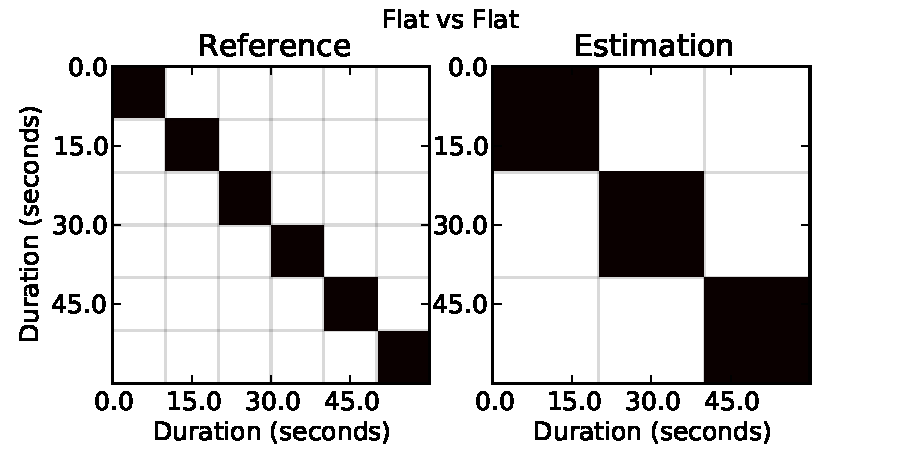
\includegraphics[width=0.94\textwidth]{plots/flat-flat.pdf}
  \end{subfigure}%
  \\
  \begin{minipage}{0.5\textwidth}
    \centering
    \vspace{10pt}
    \begin{tabular}{|c|c|c||c|c|c|}
      \hline
      \multicolumn{3}{|c||}{\textbf{SHAG}} & \multicolumn{3}{c|}{\textbf{Hit Rate (trimmed)}} \\
      \hline
      $w$ & $\mathpzc{H}_u$   & $\mathpzc{H}_o$ & $F$     & $P$     & $R$ \\
      \hline
      0.5       & 40.0   & 100   & 57.14  & 100 & 40.0 \\
      \cline{4-6}
      3         & 40.0   & 100  \\
      \cline{4-6}
      15        & 39.39  & 52.77 & \multicolumn{3}{c|}{\textbf{Median Deviations}}   \\
      \cline{4-6}
      30        & 69.49  & 49.75 & \multicolumn{2}{c|}{E2R} & 0 \\
      $\infty$  & 80.0   & 49.75 & \multicolumn{2}{c|}{R2E} & 0 \\  
      \hline
    \end{tabular}
  \end{minipage}
  \caption{Flat vs flat boundaries (top) and scores (bottom)}
  \label{fig:flat-flat}
\end{figure}

The SHAG scores for the flat annotations are shown on the left side of the table in Figure \ref{fig:flat-flat}.
Since the estimated boundaries are undersegmented, we obtain a low score for $\mathpzc{H}_u$, but a perfect score for $\mathpzc{H}_o$, since the estimation does not oversegment at any point.
These grades are exactly the same as the precision and recall values of the hit rate measure at short time windows, since we are only evaluating one level of boundaries and $P$ and $R$ also capture the amount of under and oversegmentation of the estimation respectively.
For the longer time windows, we see how the oversegmentation grade $\mathpzc{H}_o$ significantly decreases, while the undersegmented one $\mathpzc{H}_u$ increases.
This illustrates how \dots TODO

\subsection{Hierarchical vs Flat}

Here we present two different examples of a hierarchical reference against a flat estimation: flat large and small scale.
These situation may happen when we try to evaluate an algorithm that tends to undersegment (large scale) or oversegment  (small scale) against a track that is annotated hierarchically (like any track of the SALAMI dataset).
We no longer can compare our metric against the standard ones because at least one set of boundaries is hierarhichal.

\subsubsection{Flat Large Scale}

In this example we show the behavior of our grades when comparing a hierarchical reference against a flat segmentation of large scale sections.
On the top of Figure \ref{fig:hier-flatlarge} the boundaries are plotted.
Note how the estimated boundaries basically identify the highest layer of the hierarchical ones.
At the bottom of this figure we can see the grades for SHAG, which behave as expected: the oversegmentation value $\mathpzc{H}_o$ is always 100\%, since the estimated boundaries do not oversegment.
Moreover, when using small time windows (i.e. $w \leq 3$ in the figure), the undersegmented score is 0 since all the boundaries are ranked to different hierarchies at these short $w$, since the flat boundaries correspond to the higher layer of the reference ones.
However, as $w$ increases, our metric is able to correctly rank the flat boundaries against the hierarchical ones, covering the entire large scale boundaries of the top of the hierarchy, thus increasing the undersegmentation grade.

\begin{figure}
  \centering
  \begin{subfigure}{0.5\textwidth}
    \centering
    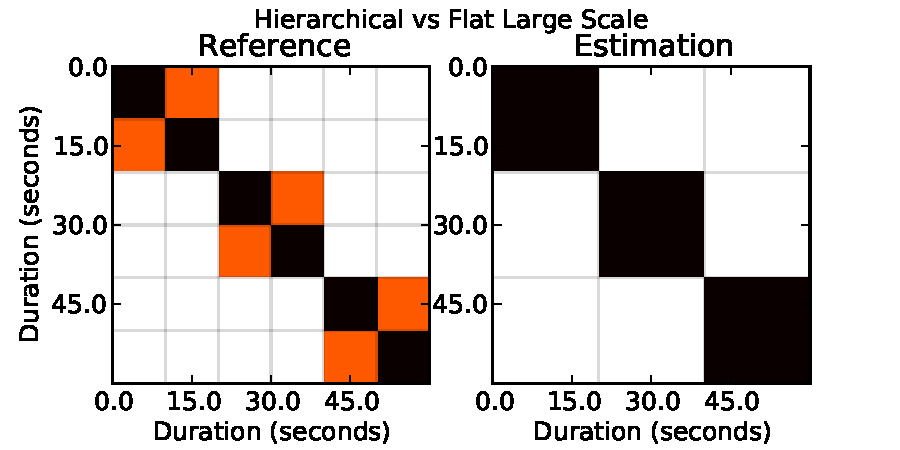
\includegraphics[width=0.94\textwidth]{plots/hier-flatlarge.pdf}
  \end{subfigure}%
  \\
  \begin{minipage}{0.5\textwidth}
    \centering
    \vspace{10pt}
    \begin{tabular}{|c|c|c|}
      \hline
      $w$       & $\mathpzc{H}_u$    & $\mathpzc{H}_o$      \\
      \hline
      0.5       & 0         & 100      \\     
      3         & 0         & 100      \\
      15        & 37.21     & 100    \\
      30        & 69.66     & 100    \\
      $\infty$  & 80.16     & 100    \\
      \hline
    \end{tabular}
  \end{minipage}
  \caption{Hierarchical vs flat large scale boundaries (top) and scores (bottom)}
  \label{fig:hier-flatlarge}
\end{figure}

\subsubsection{Flat Small Scale}

Here we analyze the behavior of SHAG in the case of a flat algorithm that tends to oversegment its estimations (therefore, the estimated segments will be smaller).
The boundaries and their results are found on the top and bottom of Figure \ref{fig:hier-flatsmall}, respectively.
Since, as in the large scale case, we are not oversegmenting, the oversegmentation grades are 100\% for all the time windows.
As opposed to the previous example, now the lower layer of the reference boundaries match exactly with the estimations, that results into perfect undersegmentation scores for the shorter time windows.
In this case, the higher the $w$, the lower these undersegmentation grades as expected, since we should not evaluate an algorithm as perfect if it only identifies one layer of the hierarchical boundaries found in the reference.


\begin{figure}
  \centering
  \begin{subfigure}{0.5\textwidth}
    \centering
    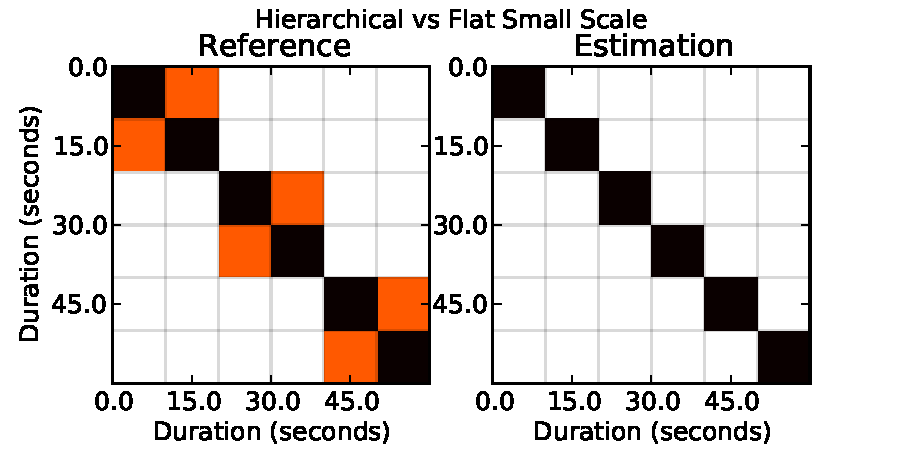
\includegraphics[width=0.94\textwidth]{plots/hier-flatsmall.pdf}
  \end{subfigure}%
  \\
  \begin{minipage}{0.5\textwidth}
    \centering
    \vspace{10pt}
    \begin{tabular}{|c|c|c|}
      \hline
      $w$       & $\mathpzc{H}_u$    & $\mathpzc{H}_o$      \\
      \hline
      0.5       & 100       & 100      \\     
      3         & 100       & 100      \\
      15        & 62.79     & 100    \\
      30        & 30.34     & 100    \\
      $\infty$  & 19.84     & 100    \\
      \hline
    \end{tabular}
  \end{minipage}
  \caption{Hierarchical vs flat small scale boundaries (top) and scores (bottom)}
  \label{fig:hier-flatsmall}
\end{figure}

\subsection{Hierarchical vs Hierarchical}

In this subsection we illustrate the behavior of SHAG with two examples of hierarchical boundaries compared to other hierarchical ones.
To start with, we see the behavior of our grades when comparing two equal hierarchical boundaries in Figure \ref{fig:hier-hier}.
As expected, SHAG returns 100\% for all the different time windows, showing how we can obtain a perfect score when the reference and estimation are exactly the same across all their layers.

\begin{figure}
  \centering
  \begin{subfigure}{0.5\textwidth}
    \centering
    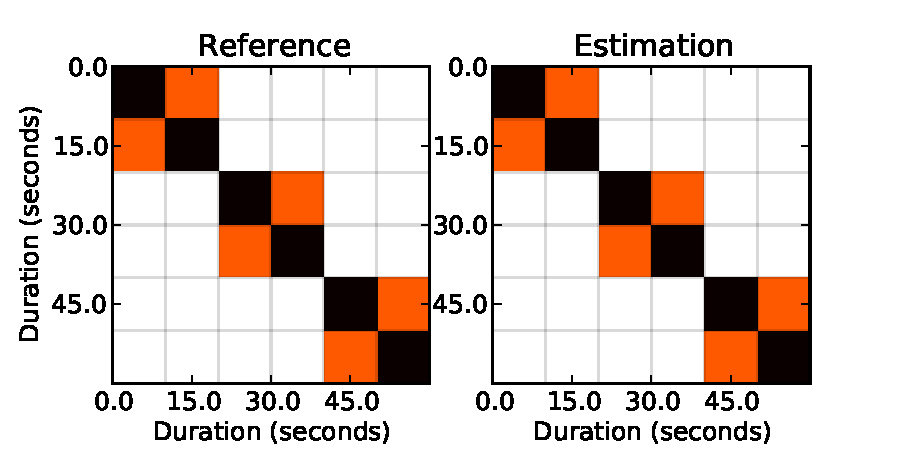
\includegraphics[width=0.94\textwidth]{plots/hier-hier.pdf}
  \end{subfigure}%
  \\
  \begin{minipage}{0.5\textwidth}
    \centering
    \vspace{10pt}
    \begin{tabular}{|c|c|c|}
      \hline
      $w$       & $\mathpzc{H}_u$    & $\mathpzc{H}_o$      \\
      \hline
      any       & 100       & 100      \\     
      \hline
    \end{tabular}
  \end{minipage}
  \caption{Hierarchical vs same hierarchical boundaries (top) and scores (bottom)}
  \label{fig:hier-hier}
\end{figure}

In Figure \ref{fig:hier-hiercomp} the boundaries (top) and the results (bottom) of two different hierarchical segmentations are shown.

\begin{figure}
  \centering
  \begin{subfigure}{0.5\textwidth}
    \centering
    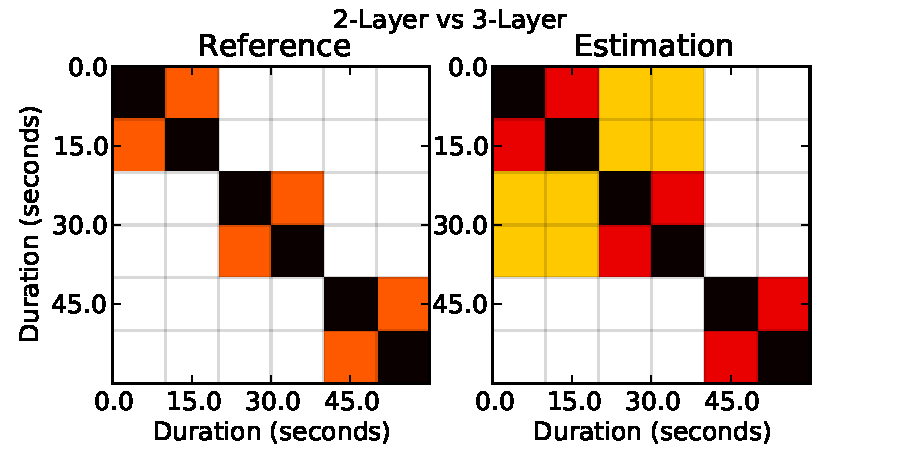
\includegraphics[width=0.94\textwidth]{plots/hier-hiercomp.pdf}
  \end{subfigure}%
  \\
  \begin{minipage}{0.5\textwidth}
    \centering
    \vspace{10pt}
    \begin{tabular}{|c|c|c|}
      \hline
      $w$       & $\mathpzc{H}_u$       & $\mathpzc{H}_o$      \\
      \hline
      0.5       & 100       & 100      \\     
      3         & 100       & 100      \\
      15        & 100       & 98.32    \\
      30        & 100       & 78.81    \\
      $\infty$  & 100       & 61.85    \\
      \hline
    \end{tabular}
  \end{minipage}
  \caption{2-layer vs 3-layer Hierarchical boundaries (top) and scores (bottom)}
  \label{fig:hier-hiercomp}
\end{figure}


\subsection{Non-synthesized Examples}

SALAMI 636 annotator 1 vs annotator 2 \ref{fig:SALAMI-SALAMI}.

\begin{figure}
  \centering
  \begin{subfigure}{0.5\textwidth}
    \centering
    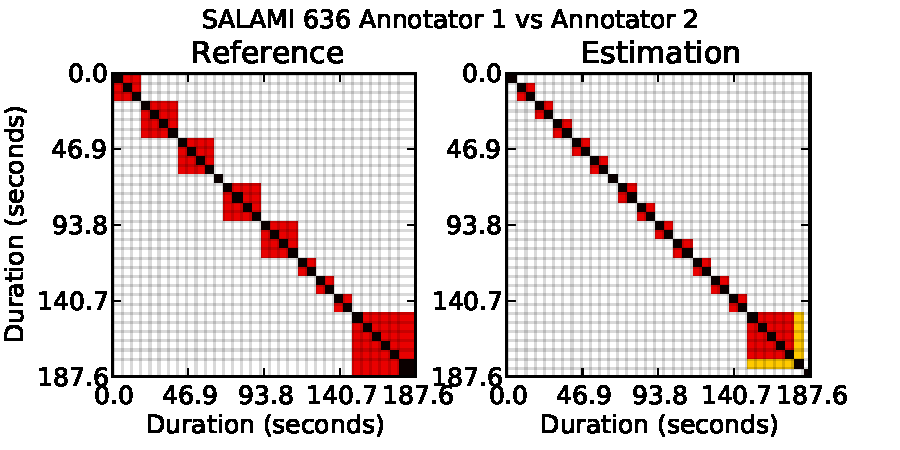
\includegraphics[width=0.94\textwidth]{plots/SALAMI-SALAMI.pdf}
  \end{subfigure}%
  \\
  \begin{minipage}{0.5\textwidth}
    \centering
    \vspace{10pt}
    \begin{tabular}{|c|c|c|}
      \hline
      $w$       & $\mathpzc{H}_u$       & $\mathpzc{H}_o$      \\
      \hline
      0.5       & 78.17       & 80.27      \\     
      3         & 95.39       & 95.27      \\
      15        & 95.65       & 90.52    \\
      30        & 95.73       & 87.98    \\
      $\infty$  & 95.75       & 95.75    \\
      \hline
    \end{tabular}
  \end{minipage}
  \caption{SALAMI 636 annotation 1 vs annotation 2 boundaries (top) and scores(bottom).}
  \label{fig:SALAMI-SALAMI}
\end{figure}

SALAMI 636 annotator 1 vs OLDA\cite{McFee2014}  output \ref{fig:SALAMI-OLDA}.

\begin{figure}
  \centering
  \begin{subfigure}{0.5\textwidth}
    \centering
    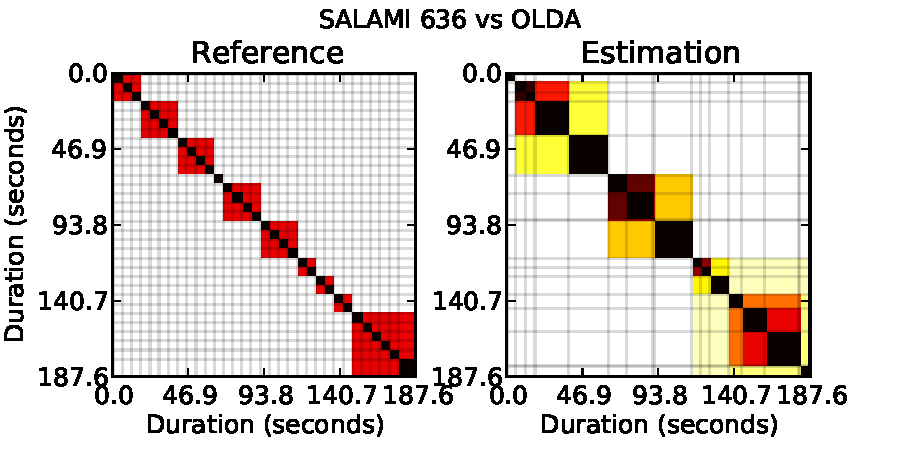
\includegraphics[width=0.94\textwidth]{plots/SALAMI-OLDA.pdf}
  \end{subfigure}%
  \\
  \begin{minipage}{0.5\textwidth}
    \centering
    \vspace{10pt}
    \begin{tabular}{|c|c|c|}
      \hline
      $w$       & $\mathpzc{H}_u$       & $\mathpzc{H}_o$      \\
      \hline
      0.5       & 14.28       & 100      \\     
      3         & 19.84       & 99.91      \\
      15        & 33.22       & 56.13    \\
      30        & 37.20       & 53.12    \\
      $\infty$  & 37.36       & 16.39    \\
      \hline
    \end{tabular}
  \end{minipage}
  \caption{SALAMI 636 annotation 1 vs OLDA output boundaries (top) and scores(bottom).}
  \label{fig:SALAMI-OLDA}
\end{figure}

%\section{Evaluating Automatic Algorithm}

%Olda\cite{McFee2014} with SALAMI.


\section{Conclusions}\label{sec:conclusions}

Extend to labeling score.

\bibliography{refs}

%\bibliography{ismir2014template}

\end{document}
